\part{Refinery and Fuels}
Crude oil (\SI{33.6}{\percent}), coke (\SI{27.2}{\percent}) and gas (\SI{23.9}{\percent}) are still the 3 main energy sources, followed by hydropower (\SI{6.8}{\percent}), nuclear power (\SI{4.4}{\percent}) and renewable energy sources (\SI{4}{\percent}).

Crude oil is the most important energy source due to its ease of extraction, wide range of applications and cheap transport.

\section{Kerogen}
Kerogen is an organic waxy material found in sedimentary rocks and formed from bacteria, decayed algae and wood.
It is the most common form of organic carbon in the earth.
Kerogen can be converted into synthetic oil at temperatures above \SI{500}{\celsius} or by hydration.
Canada (Athabasca Oil Sands) has the world's largest deposit of kerogen.
This deposit is close to the surface, making surface mining the primary method of extraction.
In this region mining of the oil sands dates back to 1967.
The worlds top reserve holders are China, United States, Argentina, Mexico, South Africa, Australia and Canada.

\subsection{Types of kerogen}
Kerogen can be divided into four different types.

\subsubsection{Typ I (Sapropelic)}
Sapropelic kerogen contains the highest amount of oil and is therefore the most promising source.
It is derived form algea and its proteins and lipids.
It contains only few cyclic or aromatic structures.
Type I kerogen has high initial hydrogen-to-carbon ratios (H/C > 1.25) and low initial oxygen-to-carbon ratios (O/C < 0.15).

\subsubsection{Type II (Planktonic)}
Planktonic kerogen is mostly based on marine organic materials.
It has a hydrogen-to-carbon ratio H/C smaller than 1.25 and initial oxygen-to-carbon ratio O/C of 0.03 to 0.18.

\subsubsection{Typ III (Humic)}
Type III kerogens are characterized by low initial H/C ratios and high initial O/C ratios.
Type III kerogens are derived from terrestrial plant matter, specifically from precursor compounds including cellulose, lignin, terpenes and phenols.
Coal is an organic-rich sedimentary rock that is composed predominantly of this kerogen type.
On a mass basis, type III kerogens generate the lowest oil yield of principal kerogen types.
It has a hydrogen-to-carbon ratio H/C smaller than 1 and initial oxygen-to-carbon ratio O/C of 0.03 to 0.3.

\subsubsection{Type IV (Residue)}
Type IV kerogen comprises mostly inert organic matter in the form of polycyclic aromatic hydrocarbons.
They have no potential to produce hydrocarbons
It has a hydrogen-to-carbon ratio H/C smaller than 0.5.

\section{Fracking}
Fracking is a method of creating, widening and stabilising cracks in the rock of a reservoir deep underground with the aim of increasing the permeability of the reservoir rocks.
This allows gases or liquids in them to flow more easily and steadily to the wellbore and be extracted.

In fracking, the fracking fluid is injected through a well under high pressure, typically several hundred bar, into the geological horizon from which it is to be extracted.
The fracking fluid is water, which is usually mixed with proppants, such as silica sand, thickeners and further additives.
Usually, several deviated wells (lateral wells) are first drilled into the reservoir by means of directional drilling, whereby the drill bit is guided parallel to the layers.
This means that the available borehole length in the reservoir is much greater, which generally increases the production yield.
Further additives are:

\begin{itemize}
    \item Gels (e.g. guar) to increase the viscosity of the fluid for better sand transport
    \item Foams (\ch{CO2} or \ch{N2}) for better transport and deposition on the proppant
    \item Acids (HCl, \ch{CH3COOH}, HCOOH, \ch{H3BO3}) for the dissolution of minerals
    \item Furthermore: Corrosion inhibitors, viscosity adjusters, biocides, fluid loss additives (preventing loss of fluid into neighboring rocks), friction minimizers
\end{itemize}

\section{Oil drilling}
Traditional methods of oil extraction have been the primary and secondary methods, which only exhaust between a quarter and half of a well’s oil reserves.
Such profligacy has been addressed by the development of a tertiary technique, more commonly known as enhanced oil recovery (EOR).

\subsection{Primary methods}
Primary oil recovery refers to the process of extracting oil either via the natural rise of hydrocarbons to the surface of the earth or via pump jacks and other artificial lift devices.
Since this technique only targets the oil, which is either susceptible to its release or accessible to the pump jack, this is very limited in its extraction potential.
Only around \SIrange{10}{20}{\percent} the well’s potential are recovered from the primary method.

\subsection{Secondary methods}
This method involves the injection of gas or water, which will displace the oil, force it to move from its resting place and bring it to the surface.
This is typically successful in targeting an additional \SI{30}{\percent} of the oil’s reserves.

\subsection{Tertiary methods (Enhanced Oil Recovery)}
Rather than simply trying to force the oil out of the ground, as did the previous two methods, enhanced oil recovery seeks to alter its properties to make it more conducive to extraction.
Tertiary methods target more than \SI{50}{\percent} of the oil’s reserves.
There are three main types of enhanced oil recovery

\subsubsection{Thermal recovery}
This is the most prevalent type of EOR and works by heating the oil to reduce its viscosity and allowing easier flow to the surface.
This is most commonly achieved by introducing steam into the reservoir, which will work to heat the oil.

\subsubsection{Gas injection}
Either natural gas, nitrogen or carbon dioxide (increasingly the most popular option) are injected into the reservoir to mix with the oil, making it more viscous, whilst simultaneously pushing the oil to the surface (similar to secondary oil recovery).

\subsubsection{Chemical injection}
Polymers or surfactans are used to free trapped oil in the well.
This is done by lowering surface tension and increasing the efficiency of water-flooding.

\section{Crude Oils}
\label{sec:crude_oils_and_products}
Crude oil contains great variety of hydrocarbons (HCs).
There are three types of molecular structures are possible straight-chain, branched-chain and ring structures (Fig.~\ref{fig:hc_structs}).

\begin{figure}[H]
    \centering
    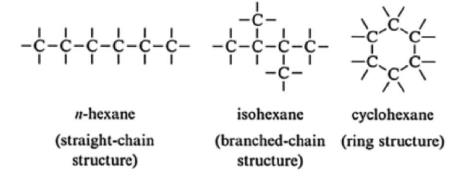
\includegraphics{Figures/HC_structures}
    \caption{Different possible hydrocarbon structures}
    \label{fig:hc_structs}
\end{figure}

\subsection{Structure of hydrocarbons}
Crude oils are complex mixtures primarily composed of hydrocarbons (HCs).
These hydrocarbons can be categorized into several groups, including saturated hydrocarbons, unsaturated hydrocarbons, aromatics, and heteroorganic compounds.

\subsubsection{Saturated hydrocarbons} They are also known as paraffins or alkanes, make up a significant portion of crude oils.
They can be further classified into normal, iso-, and cycloalkanes.
Cycloalkanes, often referred to as naphthenes, are a subgroup of saturated hydrocarbons characterized by their ring-shaped structure.

\subsubsection{Unsaturated hydrocarbons} These are in the form of olefins or alkenes.
They are not typically present in significant quantities in crude oils.
However, they can be formed during various refining processes, such as cracking and dehydrogenation.

\subsubsection{Aromatic hydrocarbons} Crude oils also contain varying amounts of aromatic hydrocarbons, including benzene, condensed polynuclear aromatics, and aromatic ring systems with various paraffinic or olefinic side chains.
Aromatics are not only naturally occurring but can also be formed in different conversion processes within the oil industry.

\subsubsection{Heteroorganic compounds}
In addition to hydrocarbons, crude oils may contain heteroorganic compounds, albeit in relatively small concentrations.
These compounds include organic molecules containing sulfur (S), nitrogen (N), and oxygen (O), as well as trace quantities of metal compounds like vanadium (V), iron (Fe), and nickel (Ni).

Crude oils can be categorized based on the types of hydrocarbons they contain, leading to three primary classifications: paraffin-based, naphthene-based, and mixed-based crude oils.

\subsection{Classification of crude oils}

\subsubsection{Based on the contained hydrocarbons}

\paragraph{Paraffin based crude oils}
These crude oils are characterized by a predominant presence of paraffinic hydrocarbons.
Within this category, the lower and medium molecular weight paraffins are particularly valuable.
They are well-suited for a wide range of catalytic conversion processes, resulting in the production of gasolines, middle distillates, and serving as essential chemical feedstocks.
On the other hand, the higher molecular weight paraffins are typically utilized as raw materials for the manufacture of lubricating oils and paraffin waxes.

\paragraph{Naphthene based crude oils}
Naphthene-based crude oils primarily consist of naphthenic, aromatic, and asphaltic hydrocarbons.
The lower and medium molecular weight components present in these crude oils are instrumental in producing high-quality gasoline components, solvents, and act as key feedstocks for the production of aromatic compounds.
In contrast, the higher molecular weight components in naphthene-based crude oils find application in the manufacturing of specialized lubricants and in the production of bitumen.

\paragraph{Mixed based crude oils}
Mixed-based crude oils represent a diverse group with an even distribution of paraffinic and naphthenic/aromatic hydrocarbons across all molecular weight ranges.
They constitute the largest class of crude oils.

\subsubsection{Based on the product fraction}

Crude oils can also be classified according to the product fractions they yield.
This classification distinguishes between light, medium, and heavy crudes, and it is primarily based on the proportions of distillates and residues within the crude oil.
In essence, the more atmospheric residues a crude oil contains, the heavier it is considered in this categorization.

\paragraph{Light crude oils} Light crude oils are characterized by a higher proportion of distillates, making them relatively easier to refine and yielding a larger quantity of valuable, lighter products such as gasoline and diesel fuel.
They are often preferred for their economic and operational advantages in the refining process.

\paragraph{Medium crude oils} These strike a balance between distillates and residues.
They contain a moderate amount of atmospheric residues and distillates.
This category can provide a diverse range of refined products, including not only gasoline and diesel but also heavier products like kerosene and lubricating oils.

\paragraph{Heavy crude oils} Heavy crude oils on the other hand, have a higher proportion of atmospheric residues, making them more challenging to refine.
They typically yield a significant amount of heavier products, including bitumen and heavy fuel oils.
These crudes are often characterized by their high viscosity and density, requiring more complex and energy-intensive refining processes.

\subsubsection{Based on sulfur content}
Crude oil classification based on sulfur content plays a pivotal role in the petroleum industry.
It categorizes crude oil into various groups, primarily focusing on the sulfur content it contains.
These categories are essential for a multitude of reasons, including pricing and environmental concerns.
Sulfur in crude oil exists in various forms, which are critical to understand for refining and processing.
It can be present in trace amounts as elemental sulfur (S), hydrogen sulfide (\ch{H2S}), and carbonyl sulfide (COS).
Additionally, sulfur can be found in organic molecules, including mercaptans, sulfides, and cyclic compounds.

Mercaptans, in particular, are primarily found in the low boiling fractions of crude oil.
When exposed to air, these mercaptans can undergo oxidation, leading to the formation of disulfides, represented as R-S-S-R.
This transformation, often facilitated by processes like the Claus process, can convert mercaptans into elementary sulfur,
which is crucial for mitigating the sulfur content in crude oil and its environmental impact during refining and utilization.

\paragraph{Low sulfur crudes}
The first and most coveted category is that of low sulfur crudes, which contain less than \SI{1}{wt\%}.
These crudes are highly desirable due to their reduced environmental impact, particularly in terms of emissions when refined and combusted.
However, the desirability of low-sulfur crudes comes at a price; they tend to be the most expensive option in the market.

\paragraph{Medium sulfur crudes}
Medium sulfur crudes ypically contain sulfur in the range of \SIrange{1}{1.5}{wt\%}.
These crudes are a compromise between environmental considerations and cost-efficiency.
They are not as environmentally friendly as their low-sulfur counterparts but offer a more economical alternative.

\paragraph{High sulfur crudes} These contain more than \SI{1.5}{wt\%} sulfur.
These crudes are known for their relatively low cost but are also the most environmentally challenging.
The higher sulfur content in these crudes can lead to increased emissions of sulfur compounds during refining and combustion, contributing to air pollution and other environmental issues.

\section{Oil products}
In general ca. \SIrange{80}{90}{\percent} of oil products are used as transportation and combustion fuels.

\subsection{Gas fuels}
Within this category, particular attention is given to Liquefied Petroleum Gas (LPG) as an exemplary case.
LPG is composed of propane, butanes, and their mixtures.
It finds application in heating and, in some countries, as a motor fuel.
Adherence to national standards is observed when assessing LPG quality, with specifications such as vapor pressure, density, and impurity levels being considered.

\subsection{Liquid fules}
The realm of liquid fuels encompasses a variety of products, each tailored for specific application.

\subsubsection{Motor gasolines}
Motor Gasolines represent products that are blended and possess a boiling range between \SIrange{40}{200}{\celsius}.
They are primarily utilized in motor car engines.
Components like light and heavy cracker and reformer gasolines, alkylates, isomerates, polymerates, pyrolysis gasoline, and LPG are incorporated.
Non-hydrocarbon additives, such as alcohols and ethers, are included to enhance renewable energy content.
Gasoline quality is contingent upon parameters like knock rating (octane number), volatility, boiling characteristics, density, oxidation stability, and lead content.

\subsubsection{Kerosenes}
Kerosenes encompass products that are tailor-made and possess a boiling range between \SIrange{150}{250}{\celsius}.
Lamp kerosene, with its long-standing tradition as a lighting and cooking oil, is characterized by specifications concerning smoke point, flash point, and volatility.
Meanwhile, jet fuels are subjected to stringent quality screening to meet aviation standards.

\subsubsection{Gas oils}
Gas oils include light and heavy gas oil fractions, often derived from straight-run and cracked sources, within a boiling range of \SIrange{200}{350}{\celsius}.
These are predominantly used as automotive diesel fuels and domestic heating fuels.

\subsubsection{Heavy fuel oils}
Heavy fuel oils comprise various grades of residual oils from distillation and conversion processes.
The correction of high density, viscosity, and sulfur content often involves blending with gas oils.
These oils are used in marine fuels (bunker fuels), power stations, and industrial furnaces.
Critical characteristics, such as density, viscosity, flash point, pour point, carbon residue, ash, water, sulfur content, and sediments, are considered.

\subsection{Non fuel applications}
Non fuel applications encompass a diverse array of uses.
LPG and light naphtha fractions are employed as feedstocks in the petrochemical industry.
Special boiling-range naphthas cater to solvents for the chemical and pharmaceutical sectors.
Paraffin waxes find applications in the paper, chemical, textile, and medical industries.
Heavy distillates are pivotal in lubricant and grease production, while heavy residues serve as raw materials for road bitumen and asphalts.
Petroleum coke and high-grade coke have a broad range of industrial applications, including electrode manufacture.

\section{Refinery}
%
\begin{figure}[H]
    \centering
    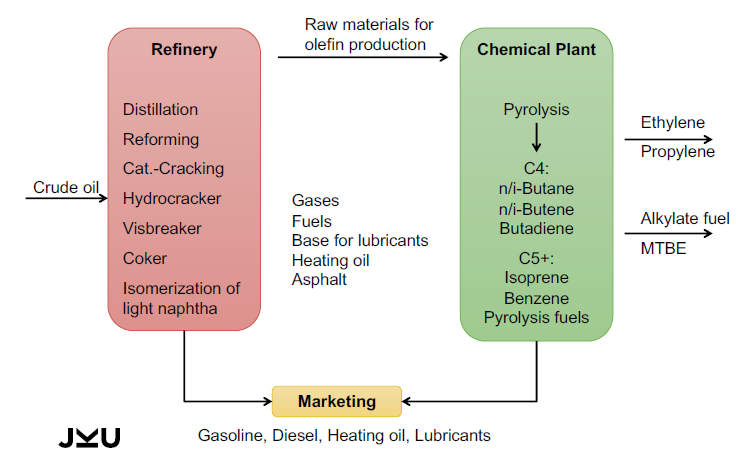
\includegraphics[scale=0.6]{refinery}
    \caption{Flow chart for refining crude oils}
    \label{fig:refinery}
\end{figure}

\subsection{Crude oil desalting}
In the process of crude oil desalting, the most commonly employed desalting unit is the electrical desalter.
This unit involves the addition of water, after which an electrical field is applied within the desalting vessel.
This action serves to disrupt saltwater-oil emulsions by inducing coalescence of the water droplets, resulting in the segregation of the water from the oil phase.
Subsequently, the oil phase is directed toward atmospheric distillation.

\subsection{Atmospheric distillation}
Atmospheric distillation involves the utilization of different boiling ranges for fractionation.
Fig.~\ref{fig:temp_yield} shows boiling overlaps, such as the case of kerosene and gas oil, and boiling gaps, as seen between heavy gasoline and kerosene or between the two gasoline fractions.
These overlaps signify a relatively suboptimal fractionation, while the presence of gaps indicates effective fractionation within the respective column section.

\begin{figure}[H]
    \centering
    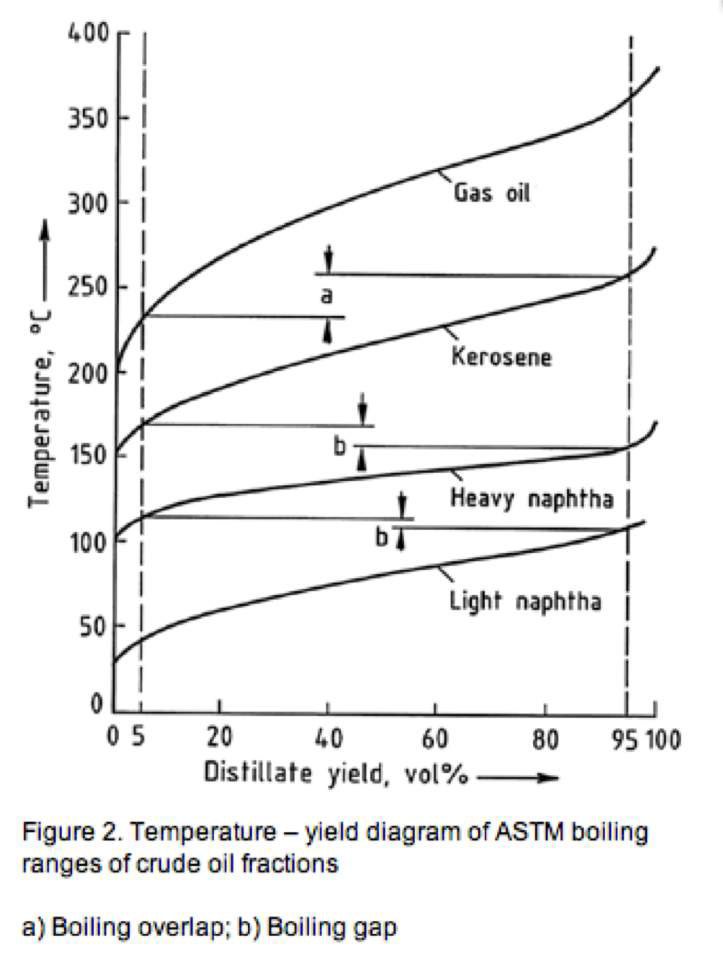
\includegraphics[scale=0.4]{temp_yield}
    \caption{Temperature-yield diagramm of ASTM (American Society for Testing and Materials) boiling ranges of crude oil fractions.}
    \label{fig:temp_yield}
\end{figure}

In the process of fractionated distillation, bell bottoms (Glockenböden) are incorporated into the fractionating column.

\subsubsection{Top product}
The vapors are condensed and subsequently separated into gas and full-range gasoline within the overhead accumulator.
A portion of the liquid gasoline is pumped back into the column as top reflux, while the remaining portion is directed towards the naphtha hydrotreater.
The gas stream, consisting of uncondensable C1-C4 hydrocarbons and \ch{H2S}, originating from the overhead accumulator, undergoes further processing within the gas treatment plant.

\subsubsection{Process water}
The process water, which is generated from the stripping steam applied to fractionator and stripper columns, is withdrawn from the sump of the overhead accumulator.
This water is subsequently treated further in a wastewater treatment plant.

\subsubsection{Side streams}
The side streams, comprising middle distillates including kerosene, light and heavy gas oil, are transferred to their respective stripper columns. 
Within these columns, the lighter constituents are separated through the injection of superheated steam.

\paragraph{Kerosene stream}
The kerosene stream from the stripper column is either pumped to a hydrotreater for the production of jet fuel or directly to storage via a heat exchanger and cooler, depending on its intended use as a blending component for diesel fuel.

\paragraph{Light gas oil stream}
The light gas oil fraction is either directed to a desulfurizing unit or pumped to storage through a heat exchanger and cooler.
It is commonly utilized for blending diesel and light heating oil.

\paragraph{Heavy gas oil stream}
The light gas oil fraction is either directed to a desulfurizing unit or pumped to storage through a heat exchanger and cooler. 
It is commonly utilized for blending diesel and light heating oil.

\subsubsection{Bottom product}
The bottom product, known as the atmospheric residue, is supplied to a vacuum fractionator to yield lubricating oil fractions.
Alternatively, it can be processed in a vacuum flasher to prepare catalytic cracker feedstock.
In some cases, this residue can serve as feedstock for various other cracking processes, including thermal and catalytic cracking, hydrocracking, or hydroconversion.

\subsection{Vacuum distillation}
In the process of vacuum distillation, the atmospheric residue resulting from crude oil distillation undergoes separation into three main components: light vacuum gas oil, heavy vacuum gas oil, and the vacuum residue.
This separation is achieved through the utilization of a vacuum flasher, a specific equipment designed for this purpose.

\subsubsection{Vacuum flasher}
The vacuum flasher, employed in this operation, is equipped with a limited number of trays.
Its primary function is to efficiently divide the atmospheric residue into one or two broad-boiling vacuum gas oils or waxy distillates.
These resulting products find essential application as feedstock for catalytic cracking (CC).
Additionally, the vacuum residue, which is another outcome of the process, serves as a valuable resource for bitumen manufacturing or as a feedstock for visbreaker processes.